\documentclass{article}

\usepackage{amsmath, amsthm, amssymb, amsfonts}
\usepackage{thmtools}
\usepackage{graphicx}
\usepackage{setspace}
\usepackage{geometry}
\usepackage{float}
\usepackage{hyperref}
\usepackage[utf8]{inputenc}
\usepackage[english]{babel}
\usepackage{framed}
\usepackage[dvipsnames]{xcolor}
\usepackage{tcolorbox}
\usepackage{textcomp}
\usepackage{listings} 


\colorlet{LightGray}{White!90!Periwinkle}
\colorlet{LightOrange}{Orange!15}
\colorlet{LightGreen}{Green!15}

\newcommand{\HRule}[1]{\rule{\linewidth}{#1}}

\declaretheoremstyle[name=Theorem,]{thmsty}
\declaretheorem[style=thmsty,numberwithin=section]{theorem}
\tcolorboxenvironment{theorem}{colback=LightGray}

\declaretheoremstyle[name=Proposition,]{prosty}
\declaretheorem[style=prosty,numberlike=theorem]{proposition}
\tcolorboxenvironment{proposition}{colback=LightOrange}

\declaretheoremstyle[name=Principle,]{prcpsty}
\declaretheorem[style=prcpsty,numberlike=theorem]{principle}
\tcolorboxenvironment{principle}{colback=LightGreen}

\setstretch{1.2}
\geometry{
    textheight=9in,
    textwidth=5.5in,
    top=1in,
    headheight=12pt,
    headsep=25pt,
    footskip=30pt
}

\begin{document}

% ====== TITLE PAGE ======
\title{ 
    \normalsize \textsc{} \\
    [2.0cm]
    \HRule{1.5pt} \\
    \LARGE \textbf{\uppercase{Seq2Seq Model for Machine Translation}} \\
    \HRule{2.0pt} \\ [0.6cm]
    \LARGE{AI6127: Deep Learning for Natural Language Processing} \\
    \vspace*{5\baselineskip}
}
\date{Submission Date: 23 April 2024}
\author{\textbf{Riemer van der Vliet} \\ 
    G2304212K}

\maketitle

\newpage

% ====== ABSTRACT ======
\section*{Abstract}
This report investigates Seq2Seq models for machine translation, analyzing their performance across various architectures. Beginning with a baseline GRU model, we explore LSTM, Bi-LSTM, attention mechanisms, and transformer encoders. Using Rouge scores, we assess translation quality. Results reveal attention-based models' superiority, particularly in bi-gram matching, showcasing their adeptness at capturing contextual nuances. Notably, Transformer models show promise but lag in convergence after two epochs, indicating potential for further improvement through extended training and hyperparameter optimization. This underscores attention mechanisms' pivotal role in advancing Seq2Seq models for translation tasks, highlighting refinement to achieve optimal performance.
\section{Introduction}
This report focuses on the implementation and comparative analysis of various Seq2Seq models for the task of machine translation. We begin with a baseline model utilizing GRU for both the encoder and decoder components, renowned for their efficiency and capacity to mitigate vanishing gradient problems common in traditional RNNs. Subsequently, we explore the substitution of GRU with LSTM in the encoder and decoder, aiming to leverage LSTM's more complex gating mechanisms for better information flow. Additionally, the implementation includes a variant with a bidirectional LSTM (Bi-LSTM) in the encoder, designed to enhance the model's context understanding by processing the input sequence in both forward and reverse directions.

\section{Methodology}
In this report the following Seq2Seq models are implemented and compared for machine translation:
\begin{itemize}
    \item Original GRU-based model.
    \item LSTM replacement for GRU.
    \item Bi-LSTM in the Encoder.
    \item Addition of the attention mechanism.
    \item Transformer Encoder integration.
\end{itemize}

\section{Experiments}
\subsection{Experimental Setup}
\subsubsection{Dataset}
This dataset serves as a practical foundation for implementing and testing seq2seq models, specifically tailored towards converting sentences from English to French. The primary source of this data is Tatoeba.org, a community-driven project aimed at providing accessible translations for various sentences across numerous languages. The Tatoeba project's extensive database allows for a broad range of applications, from language learning tools to advanced research in machine translation.

For this project, the English-French translation pairs are available through an ancillary resource, http://www.manythings.org/anki/. This facilitates the direct application of these pairs in training seq2seq models by providing a simple, structured format. Each line in the dataset file contains an English sentence followed by its French translation, separated by a tab character, making it straightforward to parse and use in training algorithms.

    ``I am cold.    J'ai froid.``

The datasets are preprocessed to remove special characters, convert text to lowercase, and tokenize the sentences. The tokenization process involves splitting the sentences into individual words, which are then used to create a vocabulary for the model. The vocabulary is a set of unique words present in the dataset, which serves as the basis for encoding and decoding text sequences during training and inference.

\subsubsection{Rouge Scores}
ROUGE scores, an acronym for Recall-Oriented Understudy for Gisting Evaluation, are a set of metrics used to evaluate the quality of text generated by a model. The ROUGE scores are based on the comparison of n-grams between the generated text and the reference text. A higher ROUGE score indicates a better match between the generated text and the reference text.

The difference between rouge1 and rouge2 is the number of words in the n-gram. Rouge1 compares unigrams, while Rouge2 compares bigrams. The fmeasure, precision, and recall are the three metrics used to evaluate the quality of the generated text.

\subsection{Results}
Here the results are discussed for the methods mentioned in Methodology.
\textbf{Baseline GRU Model}
This Gated Recurrent Unit (GRU) model serves as the baseline for comparison with other models. GRUs are known for their efficiency and ability to mitigate vanishing gradient problems common in traditional RNNs.

% === Evaluation score - Rouge score ===
% Rouge1 fmeasure:	 0.62394214
% Rouge1 precision:	 0.5904058
% Rouge1 recall:  	 0.67221373
% Rouge2 fmeasure:	 0.43355218
% Rouge2 precision:	 0.40353066
% Rouge2 recall:  	 0.47851956


\textbf{LSTM Model}
This is particularly useful in tasks where the past context is important for predicting the future, such as time series forecasting or unidirectional language translation

% on test
% === Evaluation score - Rouge score ===
% Rouge1 fmeasure:	 0.60158986
% Rouge1 precision:	 0.5764233
% Rouge1 recall:  	 0.637757
% Rouge2 fmeasure:	 0.40399328
% Rouge2 precision:	 0.38184258
% Rouge2 recall:  	 0.43781084
% =====================================

% img/LSTM_learning.png



\textbf{Bi-LSTM Model}
This approach allows the network to have both forward-looking (future) and backward-looking (past) context at every point in the sequence

% === Evaluation score - Rouge score ===
% Rouge1 fmeasure:	 0.6203933
% Rouge1 precision:	 0.5911769
% Rouge1 recall:  	 0.6619157
% Rouge2 fmeasure:	 0.42324743
% Rouge2 precision:	 0.3964009
% Rouge2 recall:  	 0.4630641

% img/LSTMBi_learning.png

\textbf{Model with Attention}
Attention allows the model to focus on different parts of the input sequence for each step of the output sequence, providing a way to dynamically weigh the input's relevance. This is especially useful in translation where the importance of input words can vary depending on the context of the output being generated. 

% === Evaluation score - Rouge score ===
% Rouge1 fmeasure:	 0.68806785
% Rouge1 precision:	 0.65075564
% Rouge1 recall:  	 0.7393444
% Rouge2 fmeasure:	 0.51409614
% Rouge2 precision:	 0.47719076
% Rouge2 recall:  	 0.5673634

% img/Attention_learning.png

\textbf{Transformer Encoder Model}

GRUs process data sequentially, which inherently limits the speed of computation, especially for long sequences. The Transformer model, addresses sequential processing limitations by employing self-attention mechanisms, enabling parallel computation and facilitating more effective learning across long sequences.

\begin{table}[ht]
    \centering
    \begin{tabular}{lcccccc}
    \hline
    \textbf{Model} & \multicolumn{3}{c}{\textbf{Rouge1}} & \multicolumn{3}{c}{\textbf{Rouge2}} \\
     & \textbf{Fmeasure} & \textbf{Precision} & \textbf{Recall} & \textbf{Fmeasure} & \textbf{Precision} & \textbf{Recall} \\
    \hline
    Baseline GRU & 0.6239 & 0.5904 & 0.6722 & 0.4336 & 0.4035 & 0.4785 \\
    LSTM & 0.6016 & 0.5764 & 0.6378 & 0.4040 & 0.3818 & 0.4378 \\
    Bi-LSTM & 0.6204 & 0.5912 & 0.6619 & 0.4232 & 0.3964 & 0.4631 \\
    Attention model & 0.6881 & 0.6508 & 0.7393 & 0.5141 & 0.4772 & 0.5674 \\
    Transformer model & 0.2069 & 0.2604 & 0.1793 & 0.1209 & 0.1615 & 0.1029 \\
    \hline
    \end{tabular}
    \caption{Evaluation scores - Rouge metrics for the different models}
    \label{table:rouge_scores}
\end{table}

\begin{figure}[htbp]
    \centering
    \begin{minipage}[t]{0.19\textwidth}
        \centering
        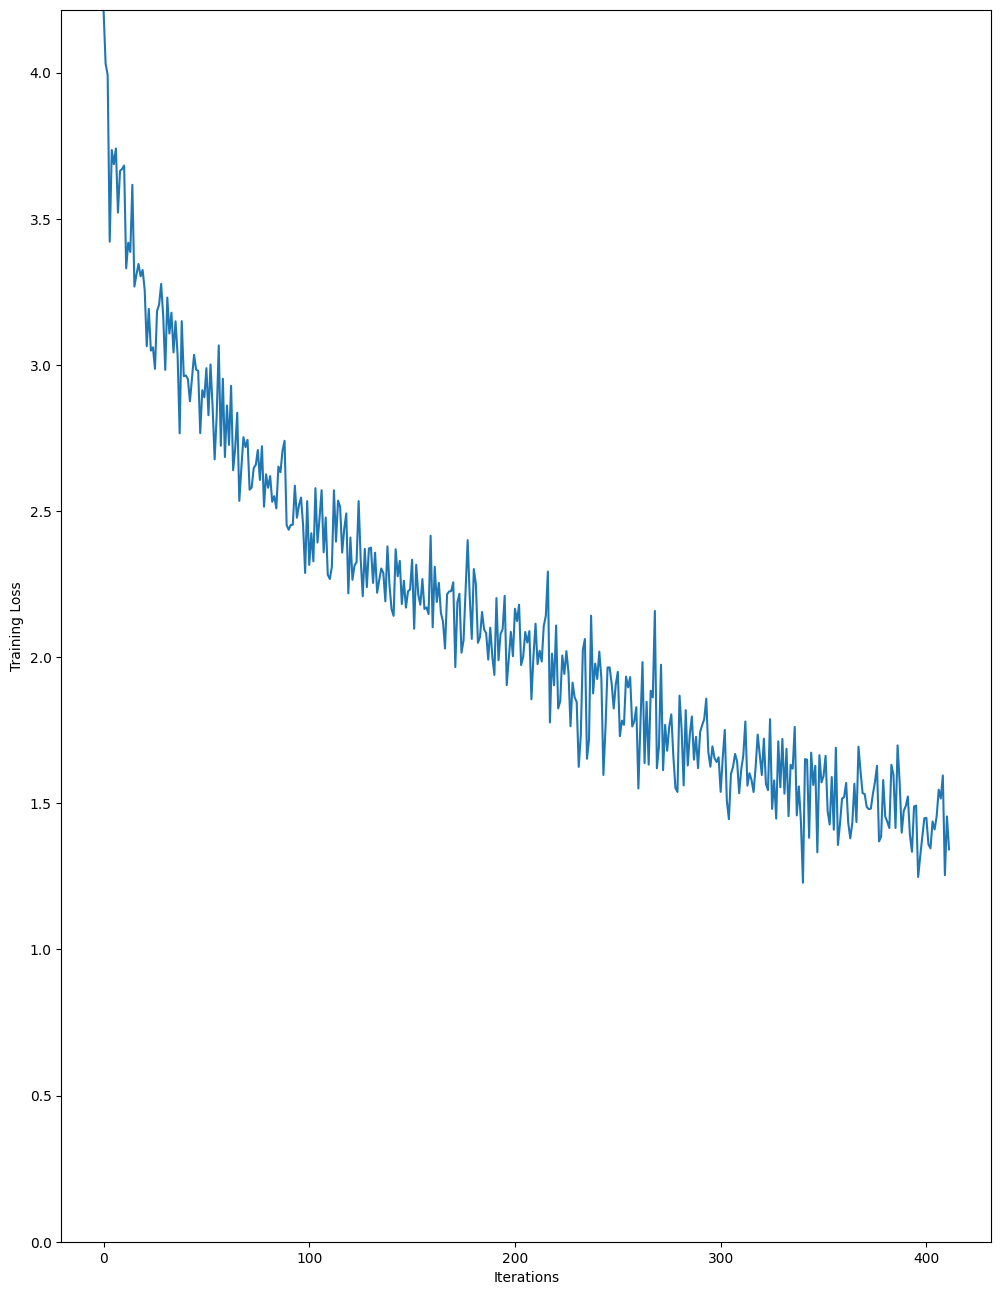
\includegraphics[width=\textwidth]{img/GRU_learning.png} \\
        \caption{GRU}
        \label{fig:gru}
    \end{minipage}
    \hfill
    \begin{minipage}[t]{0.19\textwidth}
        \centering
        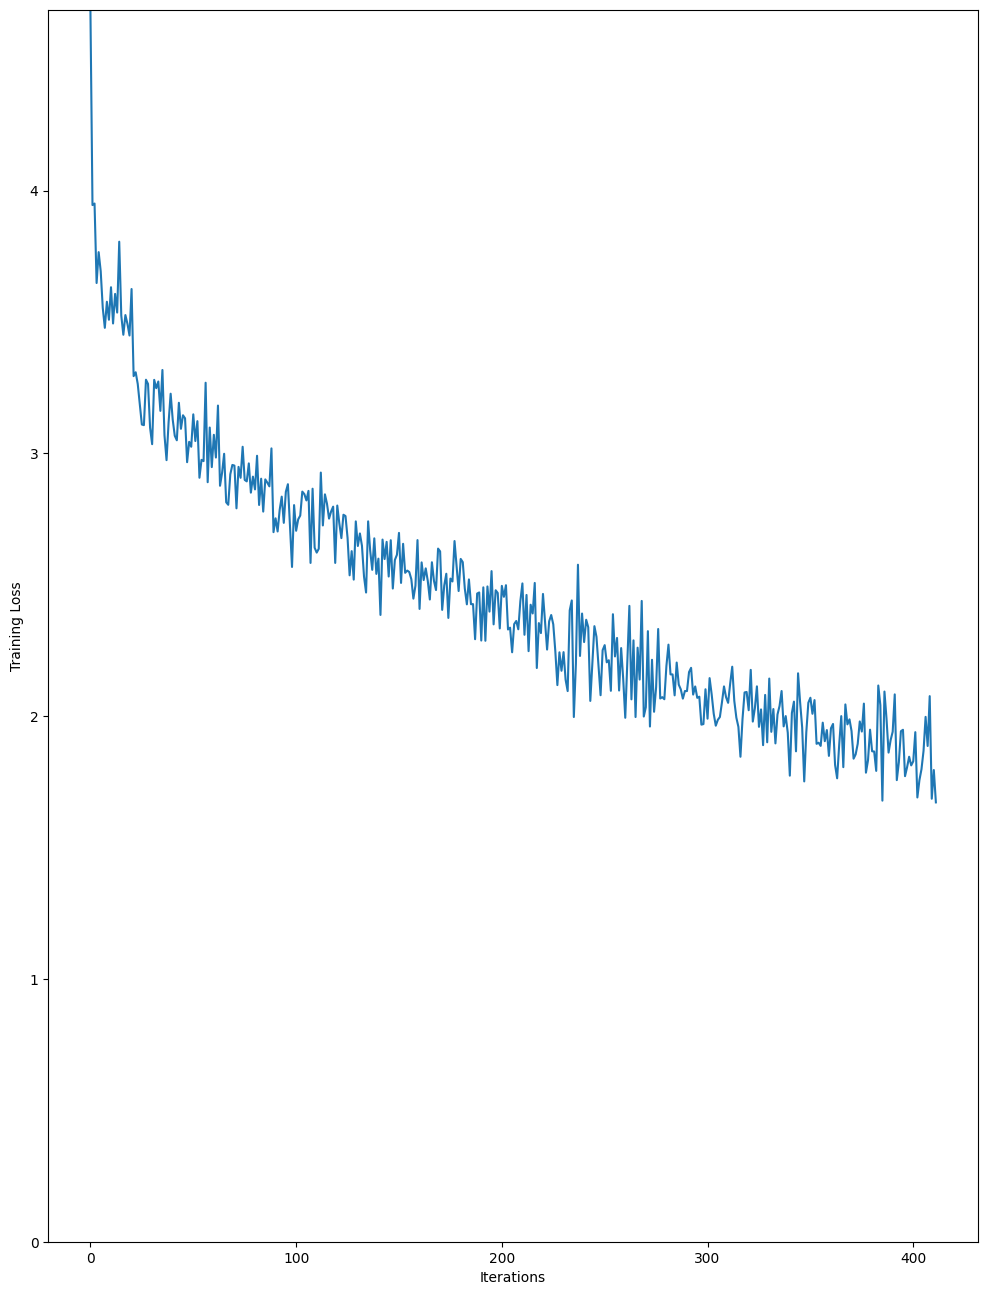
\includegraphics[width=\textwidth]{img/LSTM_learning.png} \\
        \caption{LSTM}
        \label{fig:lstm}
    \end{minipage}
    \hfill
    \begin{minipage}[t]{0.19\textwidth}
        \centering
        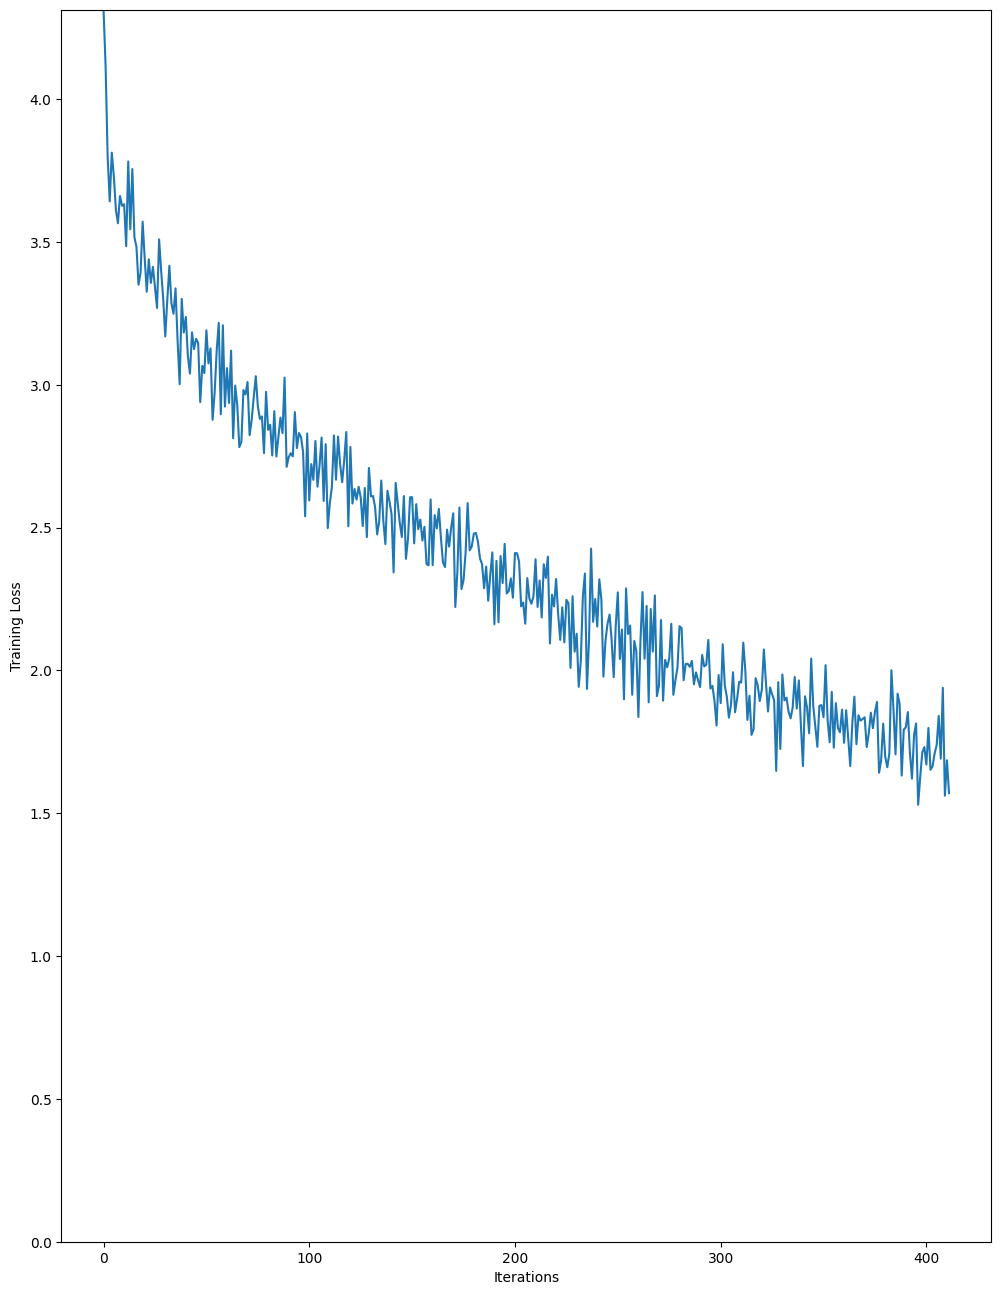
\includegraphics[width=\textwidth]{img/LSTMBi_learning.png} \\
        \caption{Bi-LSTM}
        \label{fig:bilstm}
    \end{minipage}
    \hfill
    \begin{minipage}[t]{0.19\textwidth}
        \centering
        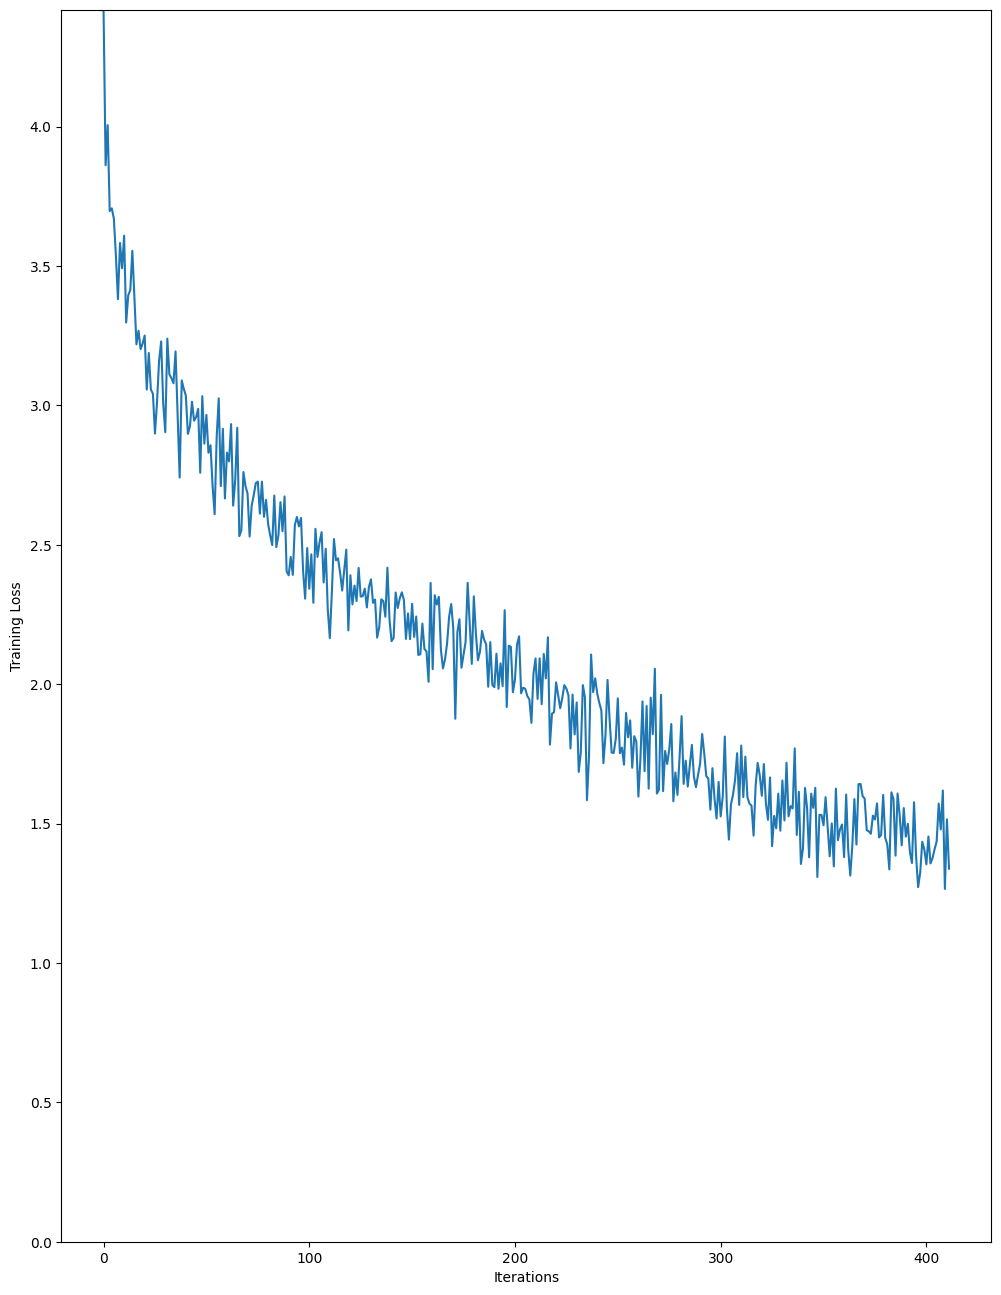
\includegraphics[width=\textwidth]{img/Attention_learning.png} \\
        \caption{Attention}
        \label{fig:attention}
    \end{minipage}
    \hfill
    \begin{minipage}[t]{0.19\textwidth}
        \centering
        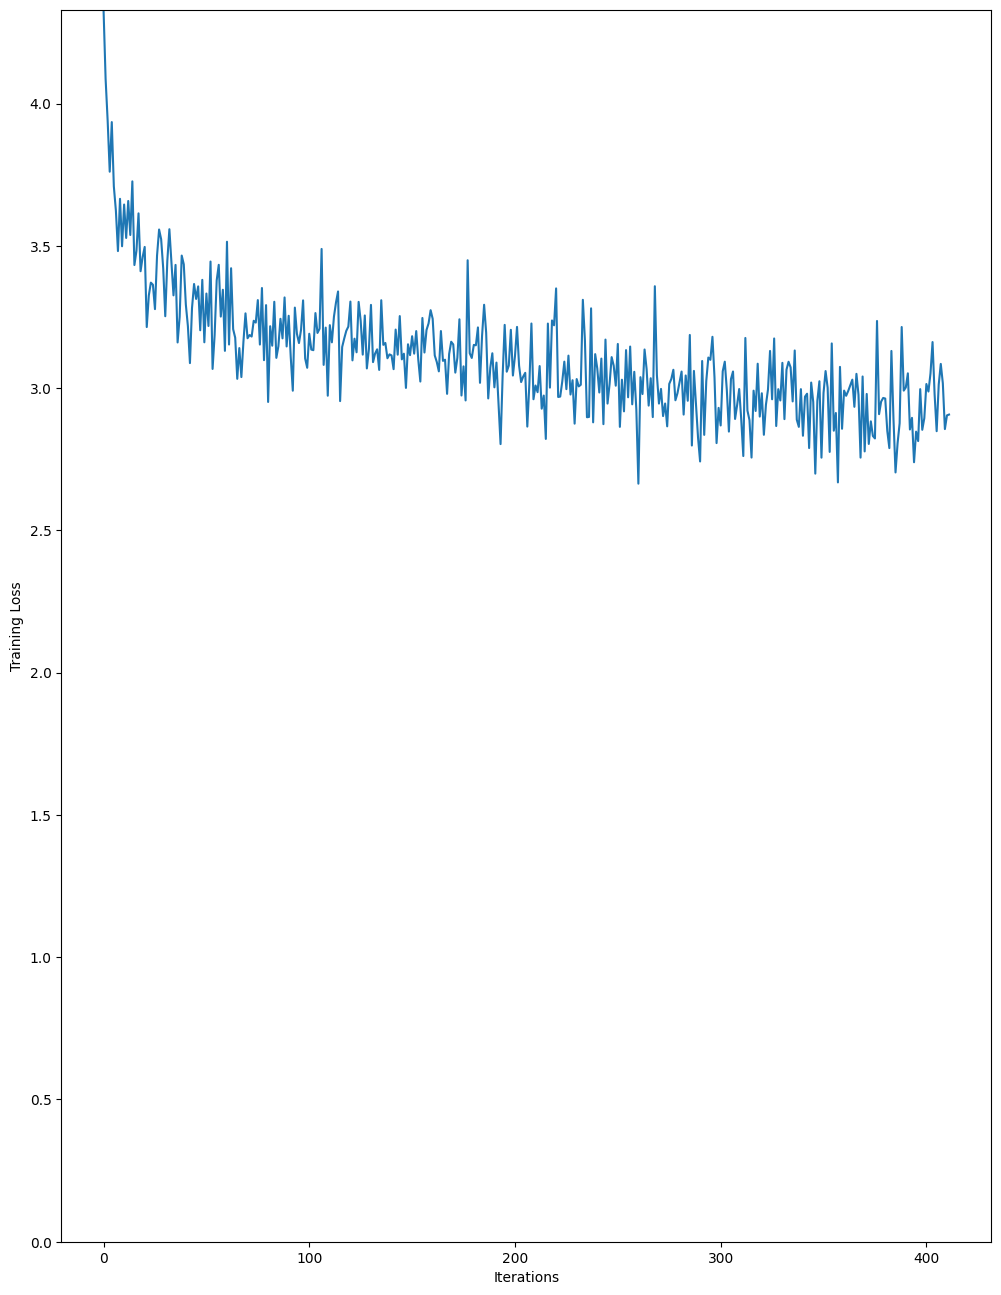
\includegraphics[width=\textwidth]{img/Transformer_learning.png} \\
        \caption{Transformer}
        \label{fig:transformer}
    \end{minipage}
    \caption{Comparison of Seq2Seq Models training over 2 epochs.}
    \label{fig:seq2seq_models}
\end{figure}

\section{Discussion}

As you can see in table \ref{table:rouge_scores}, the model with attention outperforms the other models in terms of Rouge scores. This is expected as the attention mechanism allows the model to focus on different parts of the input sequence for each step of the output sequence, providing a way to dynamically weigh the input's relevance. This is especially useful in translation where the importance of input words can vary depending on the context of the output being generated.

It's worth noting that the attention model scores particularly high on the Rouge2 set, which implies that attention has some additional benefits when it comes to bi gram matching. That none of the other models possess.

When it comes to learning there should be considered hyperparameter optimization, but as can be seen in \ref{fig:gru}, \ref{fig:lstm}, \ref{fig:bilstm}, \ref{fig:attention}, and \ref{fig:transformer} the models are learning at a similar pace and all converging. However, the transformer model, after 2 epochs, seems to be much further removed from converging. Which implies more epochs would benefit this model in particular. 

\section{Conclusion}

In conclusion, the comparative analysis of Seq2Seq models for machine translation reveals that the model incorporating attention mechanism outperforms others in terms of Rouge scores. This superiority is attributed to the attention mechanism's capability to dynamically weigh the relevance of input words based on the context of the output being generated. Particularly, the attention model excels in bi-gram matching, which is evident from its high Rouge2 score compared to other models.

Moreover, while all models exhibit similar learning trends and convergence patterns, the transformer model appears to lag in convergence after 2 epochs. This suggests that further training epochs would likely benefit the transformer model, emphasizing the importance of hyperparameter optimization for optimal performance across all models.

In essence, the study underscores the significance of attention mechanism in enhancing the performance of Seq2Seq models for machine translation tasks, and it highlights the potential for further improvements through continued training and fine-tuning of hyperparameters.
\section{References}
\bibliographystyle{IEEEtran}
% Include your references here

\section{Appendix}

Codebase can be found under `./src` in the git repository \url{https://github.com/Riemer1818/AI6127-dNLP-Ass2}.

\end{document}